\documentclass[final,t,overlay, xcolor=table, sans, mathserif]{beamer}
\mode<presentation>
{
\usetheme{UCL}
}
\usepackage[orientation=landscape,size=a0,scale=1.15, debug]{beamerposter}
% \usepackage[orientation=landscape,size=custom, width=141, height=100,scale=1.2, debug]{beamerposter}
% \usepackage[orientation=landscape,size=custom,width=178,height=88.8,scale=1.6]{beamerposter}

% additional packages
\usepackage{tikz}
\usepackage{paralist}
\setdefaultleftmargin{4.5em}{}{}{}{}{}
\usepackage{array}
\usepackage[english]{babel}
\usepackage[latin1]{inputenc}
\usepackage{wrapfig}
\usepackage{amsmath}
\usepackage{natbib}
\usepackage{multirow}
%\usepackage[pdftex]{graphicx}
\usepackage{epstopdf} 
\usepackage{xcolor}
\usepackage{tcolorbox}
%\usepackage{svg}
%\usepackage[inkscape={/Applications/Inkscape.app/Contents/Resources/bin/inkscap??e -z -C}]{svg}

%\usepackage{kerkis}
%\usepackage{kmath}


% additional settings
\setbeamerfont{itemize}{size=\normalsize}
\setbeamerfont{itemize/enumerate body}{size=\normalsize}
\setbeamerfont{itemize/enumerate subbody}{size=\normalsize}

\pdfpageattr{/Group << /S /Transparency /I true /CS /DeviceRGB>>}


%\graphicspath{{fig/}}

% Display a grid to help align images
%\beamertemplategridbackground[1cm]

\title{Performance of synchrony and spectral-based features in early seizure detection:\\
exploring feature combinations and effect of latency.}
\author[Adam \& Soldado-Magraner]
{Vincent Adam$^1$, Joana Soldado Magraner$^1$, Wittawat Jitkrittum$^1$, Heiko Strathmann$^1$,
Balaji Lakshminarayanan$^1$, Alessandro Davide Ialongo$^1$, Gergo Bohner$^1$, Ben Dongsung Huh$^1$,\\
 Lea Goetz$^2$, Shaun Dowling$^3$, Iulian Vlad Serban$^3$, Matthieu Louis$^3$}
\institute[UCL]{The Gatsby Computational Neuroscience Unit$^1$, Wolfson Institute for Biomedical Research$^2$,
The Centre for Computational Statistics and Machine Learning$^3$ (CSML), UCL, London, UK.}

\date[IWSP7 2015]{IWSP7 2015}


\begin{document}
\begin{frame}{}


\begin{columns}[t]
%%%%%%%%%%%%% BEGIN COLUMN ONE %%%%%%%%%%%%%%%%%%%%%%%%%%%%%%%%%%%%%%%%%%%%
\begin{column}{.35\linewidth}



\begin{block}{Motivation and goals}
\begin{itemize}
\item In order for a responsive neurostimulation device to successfully stop seizures,
a seizure must be detected and electrical stimulation applied as early as possible.
\item Availability of large scale iEEG datasets and recent advances in machine learning
 techniques make it possible to design efficient algorithms for this purpose.
\item The success of detecting seizures from recorded iEEG signals relies heavily on
 extracting discriminative features in the data which characterize different brain states.
\end{itemize}
\end{block}



\begin{block}{Previous work on detection}
\begin{itemize}
\item which features
\item which classifiers
\item pros and cons, what's mising?
\end{itemize}
\end{block}


\begin{block}{Our algorithm, in a nutshell}
In this study, we combine a small set of features based on neural synchrony, including fitted parameters of
multivariate autoregressive (VAR) models and pairwise phase-locking-values (PLV), and single channel features based on
spectral energy (SE). We pair these features with the state-of-the-art random forest classifier to yield an algorithm
which is able to accurately identify ictal iEEG data segments and detect early periods of the seizures
(latency from seizure onset\textless15s). \\

\centering

\begin{minipage}[t]{0.95\linewidth}
\begin{tcolorbox}[title=1. Preprocessing]
The signal was downsampled to 400Hz and low pass filtered with cutoff freq 400Hz. Electrical noise in the band $59-61Hz$ was also removed.
\end{tcolorbox}
\end{minipage}

\begin{minipage}[t]{0.95\linewidth}
\begin{tcolorbox}[title=2. Feature extraction]
The aim is to obtain a set of parameters (feature vectors) which summarize the task-relevant statistics of the iEEG data.
\qquad \\

\begin{itemize}
\item {\bf Spectral energy (SE)} \\
Squared modulus of the signal's Fourier transform. Energy below $f_{max}$ was averaged into $N_{bands}$ contiguous
bands of spectral width $\lfloor f_{max}/N_{bands}\rfloor$. \\
\qquad \\

\item {\bf Phase Locking Value (PLV)} \\
For each channel i, the instantaneous phase $\phi_{i}^{a}(t)$ of the analytical signal $x_{i}^{a}(t)$
of the time series $x_{i}(t)$ is extracted. Then, for each pair (i,j) of channels,
we compute: \\
$PLV_{ij}=\left|\frac{1}{T}\sum_{t}e^{i(\phi_{i}^{a}(t)-\phi_{j}^{a}(t))}\right|$ \\
\qquad \\

\item {\bf Vector autoregressive (VAR$\left[\tau\right]$) models} \\
The signal was modelled as: \\
$x_{t}=\sum_{k=1}^{\tau}A_{k}x_{t-k}+\epsilon_{t}, \epsilon\sim\mathcal{N}(0,Q)$ \\
The learned parameters $[A_{1},A_{2},...,A_{\tau},Q]$ were taken as features. \\
\qquad \\

\end{itemize}
\end{tcolorbox}
\end{minipage}


\begin{minipage}[t]{0.95\linewidth}
\begin{tcolorbox}[title=3. Clasification]
Random Forest classifier trained individually for each subject.
\end{tcolorbox}
\end{minipage}

\end{block}



\end{column}
%%%%%%%%%%%%% BEGIN COLUMN TWO %%%%%%%%%%%%%%%%%%%%%%%%%%%%%%%%%%%%%%%%%%%%
\begin{column}{.65\linewidth}

 
\begin{block}{The task}
Multi-channel iEEG data from human patients and dogs with epilepsy was provided by the UPenn-Mayo Clinic
Seizure Detection Challenge, hosted on kaggle.com, which was sponsored by the American Epilepsy Society. \\
In this work, we aimed to solve two tasks:
\begin{itemize}
\item I. We evaluate the accuracy of the classifier in seizure detection and early seizure detection. Furthermore, we
analyse the importance of the different features for classification performance.
\item II. We compare the estimated probabilities of seizure and early seizure against latency to characterize how accuracy
changes as the seizure progresses.
\item III. We repeat the same analysis as in I, but on a seizure prediction task.
\end{itemize}
\end{block}

\vspace{-1.2cm}
\begin{columns}
\column{0.49\textwidth}
\begin{block}{Results I. Seizure \& early seizure detection performance}
\begin{columns}
\column{0.49\textwidth}
\vspace{-1cm}
\begin{figure}
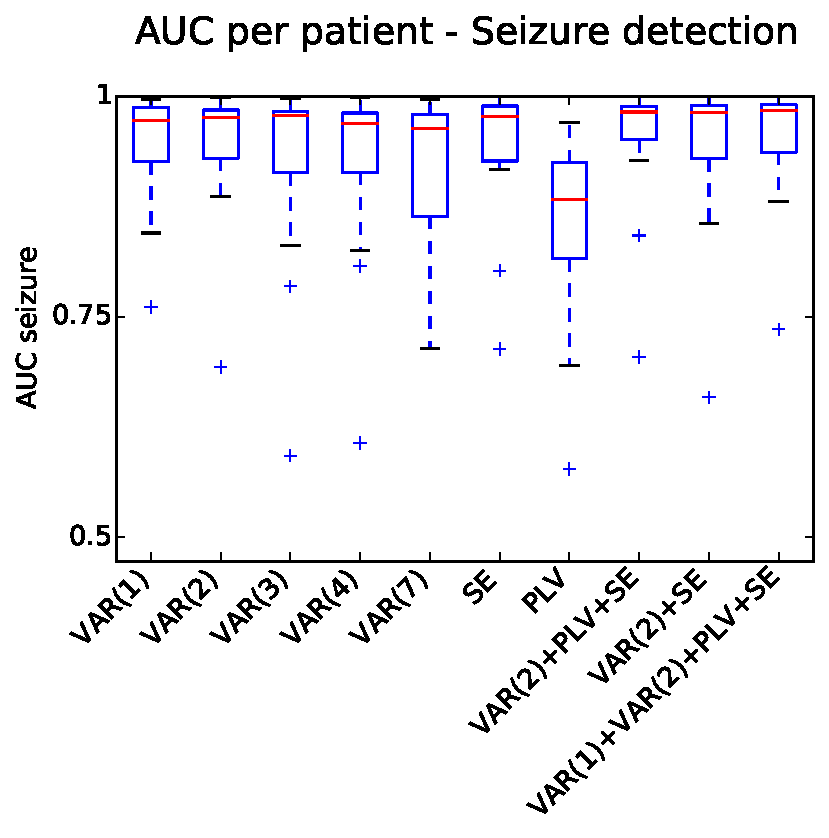
\includegraphics[width=1\textwidth]{figures/kaggle_2_train_test_seizure.pdf}
\end{figure}
\column{0.49\textwidth}
\vspace{-1cm}
\begin{figure}
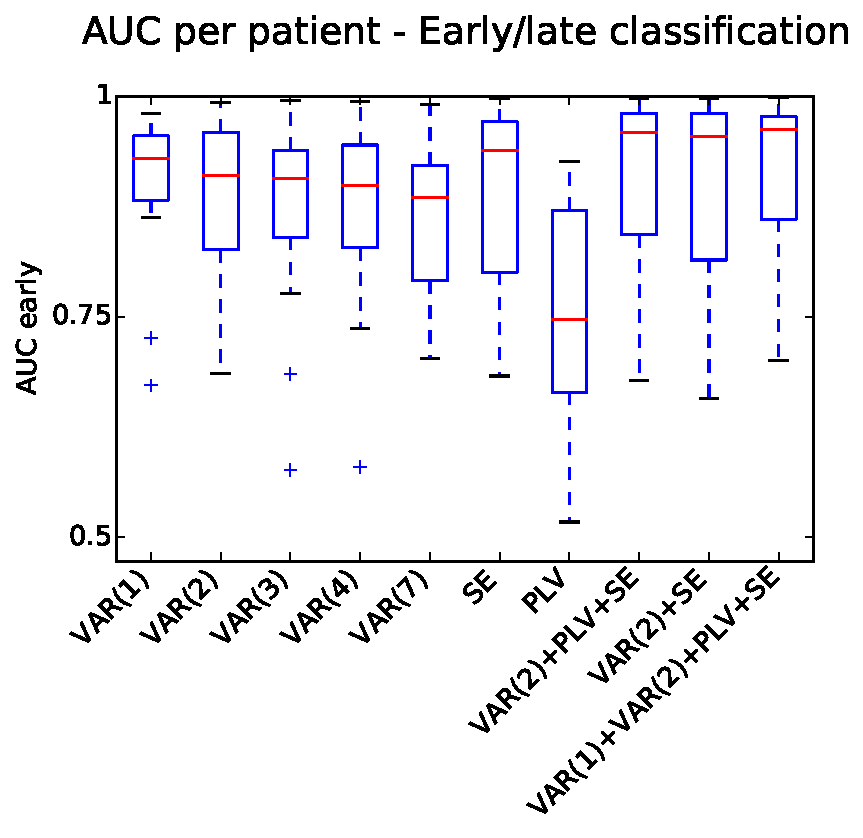
\includegraphics[width=1\textwidth]{figures/kaggle_2_train_test_early.pdf}
\end{figure}
\end{columns}
\end{block}
\column{0.49\textwidth}
\begin{block}{Results III. Seizrue prediction performance}
\begin{columns}
\column{0.49\textwidth}
\vspace{-1cm}
\begin{figure}
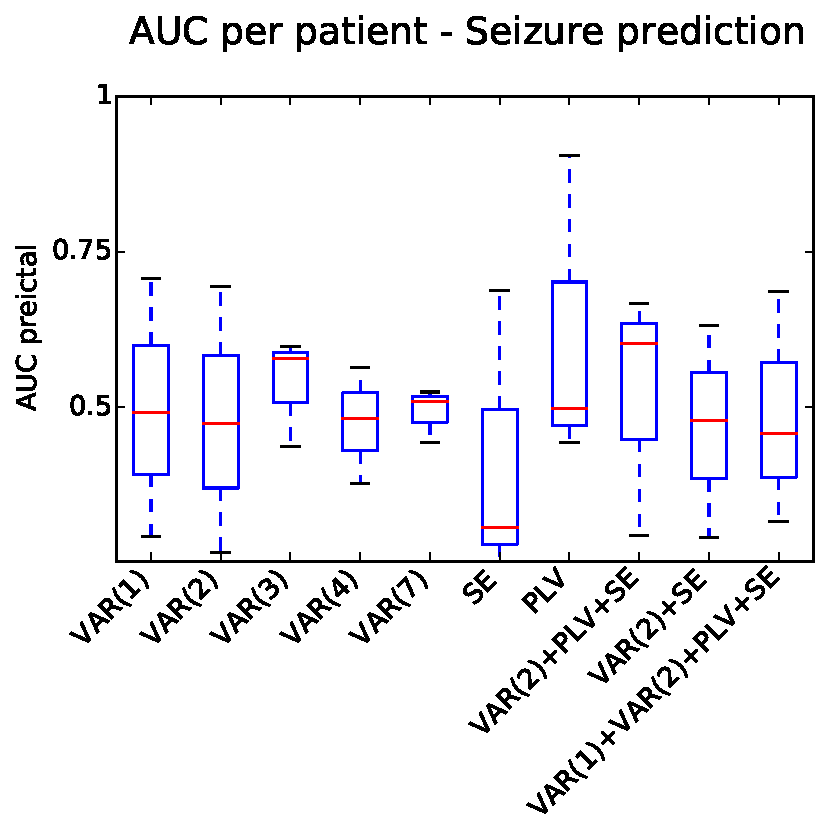
\includegraphics[width=1\textwidth]{figures/kaggle_prediction_seizure.pdf}
\end{figure}
\column{0.49\textwidth}
\begin{itemize}
\item We run the same analysis
\item Overall performance drops significantly
\end{itemize}
\end{columns}
\end{block}
\end{columns}

\begin{columns}
\column{0.49\textwidth}
\begin{block}{Results II. Latency. Example 1.}
\begin{figure}
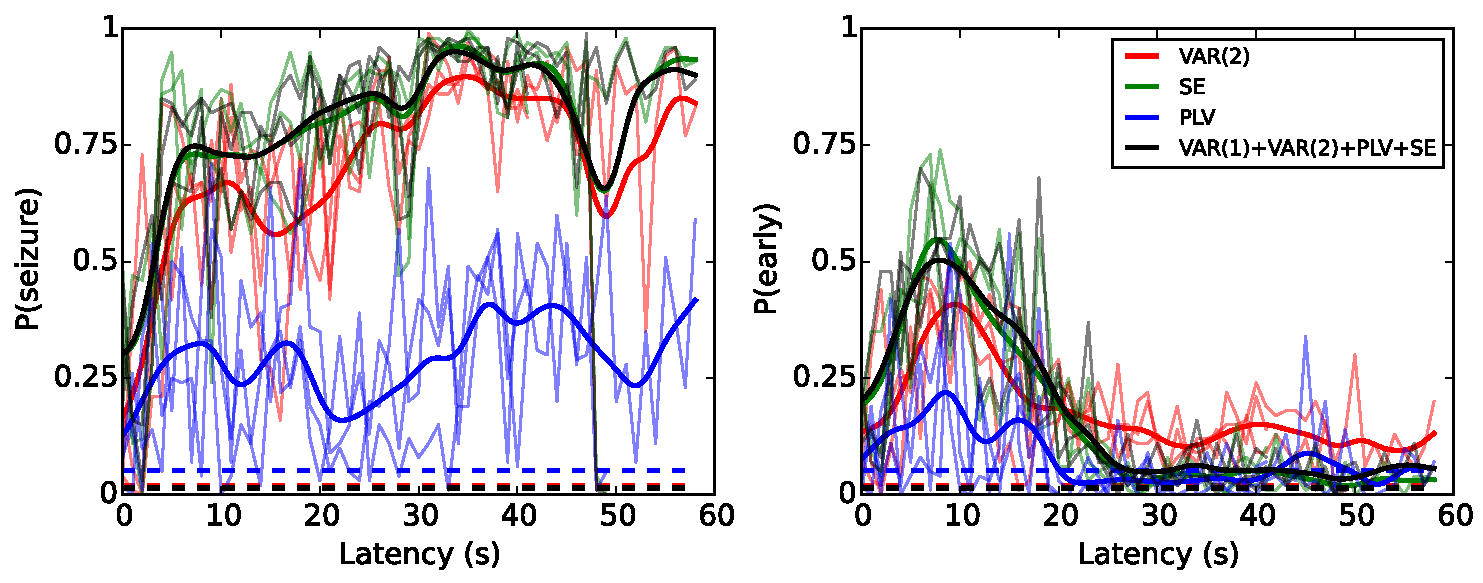
\includegraphics[width=0.85\textwidth]{figures/Patient_2_latency.pdf}
\end{figure}
\end{block}
\column{0.49\textwidth}
\begin{block}{Results II. Latency. Example 2.}
\begin{figure}
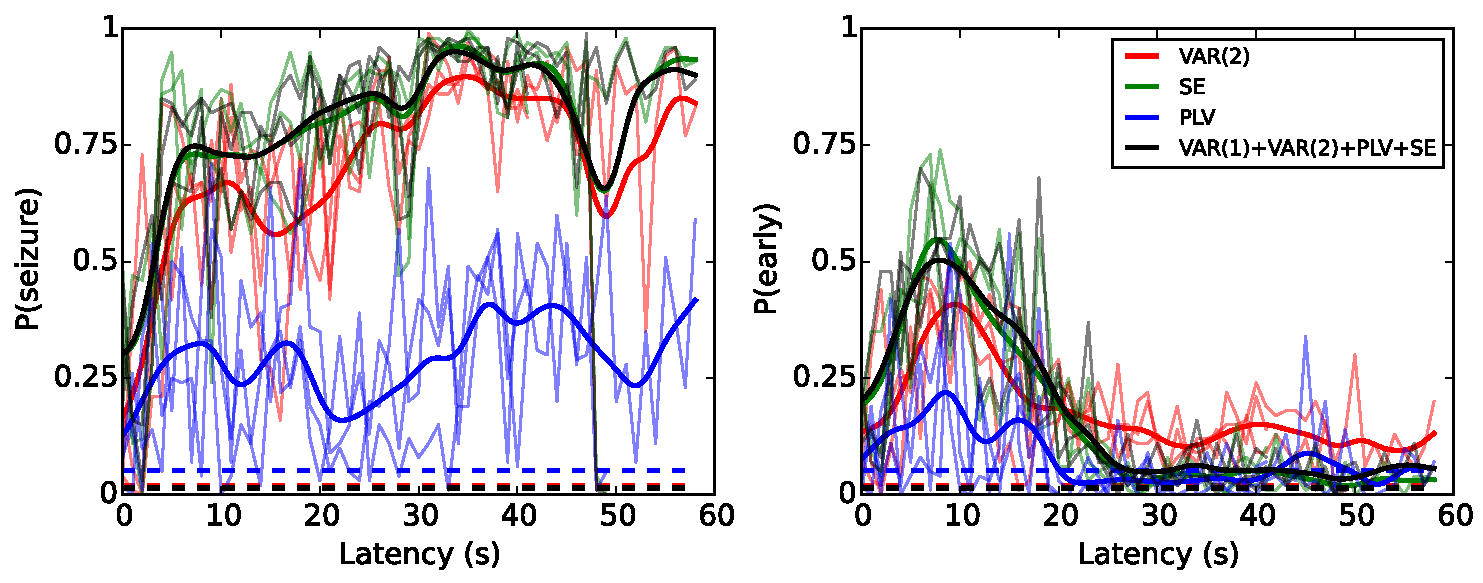
\includegraphics[width=0.85\textwidth]{figures/Patient_2_latency.pdf}
\end{figure}
\end{block}
\end{columns}

\begin{columns}
\column{0.49\textwidth}
\begin{block}{Results II. Latency}
\centering
Mean performance across subjects, for different feature combinations.
\begin{figure}
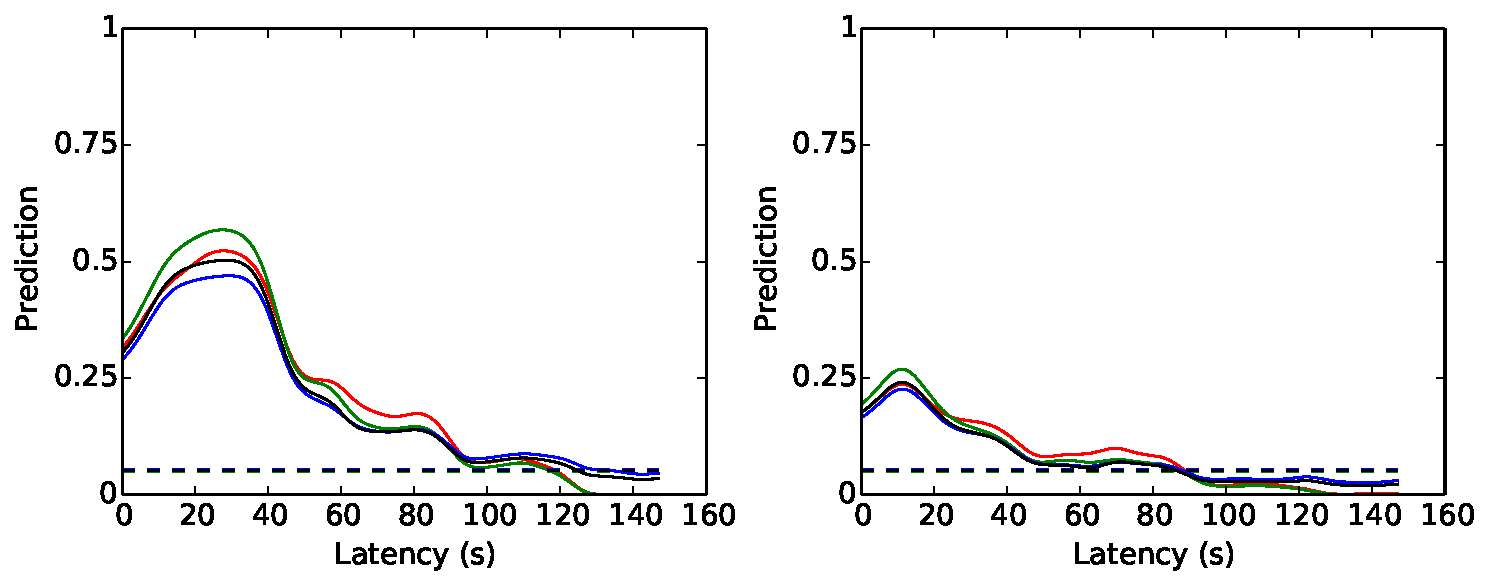
\includegraphics[width=0.85\textwidth]{figures/all_latency.pdf}
\end{figure}
\end{block}
\column{0.49\textwidth}
\begin{block}{Conclusions}
\begin{itemize}
\item features extracted with VAR models beyond 2nd order do not improve classification performance
\item A combination of SE+VAR+PLV achieves the best results in both tasks
\item data segments are more confidently classified as ictal as seizure progresses (latency)
\item Best features for prediction are...
\item Compare performance vs VAR degree. In detection clearly decreases, in prediction...
\end{itemize}
\end{block}
\end{columns}



\end{column}
%%%%%%%%%%%%% END COLUMNS %%%%%%%%%%%%%%%%%%%%%%%%%%%%%%%%%%%%%%%%%%%%
\end{columns}


\end{frame}
\end{document}
